\documentclass[xcolor=dvipsnames]{beamer}
\usepackage{graphicx,epstopdf}
\usepackage{fancyhdr}
\usepackage{cite}
\usepackage{graphicx, epstopdf}
\usepackage{amsmath}
\usepackage{array}
\usepackage{epsfig}
\usepackage{amssymb}
\usepackage{subfigure}
\usepackage[ruled, lined,linesnumbered]{algorithm2e}
\usepackage{algorithmic}
\usepackage{tabularx}
\usepackage{rotating, boxedminipage}
\usepackage{rotating,multirow}
\usepackage{float}
\usepackage{wrapfig}
\usepackage{algorithm2e}
\usetheme{Boadilla}
\usecolortheme[named=Blue]{structure}
\setbeamertemplate{items}[square]
\setbeamertemplate{caption}[numbered]
\setbeamertemplate{caption}[small]
\usepackage[absolute,overlay]{textpos}
\newenvironment{reference}[2]{
  \begin{textblock*}{\textwidth}(#1,#2)
     \bgroup\fontsize{6pt}{\baselineskip}\selectfont\color[RGB]{0,112,192}}{\egroup\end{textblock*}}

\begin{document}
    \title[Real-Time Face Recognition]{Real-Time Face Recognition}
    \author[Rajat Dubey]{Rajat Dubey}
    \institute[GECB]{Government Engineering College Bikaner}
    \logo{
\includegraphics[height=0.5cm,width=3.0cm]{Ecb_logo}\vspace{230pt}}
    \date{March 2018}
    \begin{frame}
        \titlepage
    \end{frame}
    \setbeamertemplate{section in toc}[square]
    
    \begin{frame}
    \frametitle{Real-Time Face Recognition}
    \begin{figure}[H]
    \graphicspath{{figs/}}
    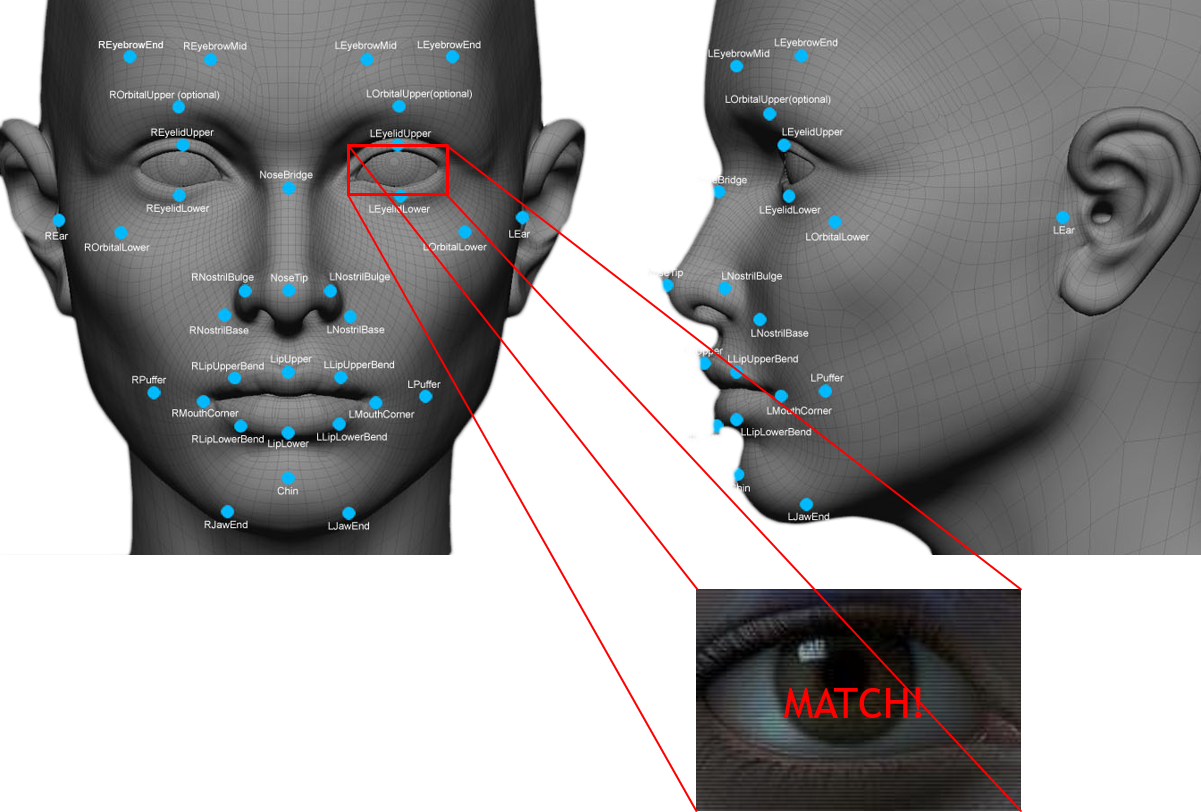
\includegraphics[width=1.0\textwidth]{Facial.png}
    \caption{}
    \end{figure}
    \end{frame}
    
    \begin{frame}
        \frametitle{Table of Contents}
        \tableofcontents
    \end{frame}

    \section{Face Recognition}
    \begin{frame}
      \frametitle{Content for Section \thesection}
      \tableofcontents[currentsection]
    \end{frame}

    \begin{frame}
    \frametitle{Face Recognition}
    \textbf{Define}: Face recognition system is a computer application for automatically identify or verifying a person from a digital image or video frame. In this system automatically searching of faces from the face databases, typically resulting in a group of facial images ranked by computer evaluated similarity.\\
    "Face Recognition" generally involves two stages:
    \begin{itemize}
    \item Face Detection, where a photo is searched to find any face (shown here as a green rectangle), then image processing cleans up the facial image for easier recognition.
    \item Face Recognition, where that detected and processed face is compared to a database of known faces, to decide who that person is (shown here as red text).
    \end{itemize}
    \end{frame}


    \section{Why real-time face recognition?}
    \begin{frame}
      \frametitle{Content for Section \thesection}
      \tableofcontents[currentsection]
    \end{frame}

    \begin{frame}
    \frametitle{Why Real-Time Face Recognition?}
    
    \begin{block}{Security:}
    \begin{itemize}
    \item Fight Terrorism
    \item Find Fugitives
    \end{itemize}
    \end{block}
    
    \begin{block}{Personal information access:}
    \begin{itemize}
    \item ATM
    \item Computer System
    \item Home access (no keys or passwords)
    \item Any other application that would want personal identification
    \end{itemize}
    \end{block}
    
    \begin{itemize}
    \item Improved human-machine interaction
    \item Personalized advertising
    \item Beauty Search
    \end{itemize}
    \end{frame}

 
    \section{What is difficult about real-time face recognition?}
    \begin{frame}
      \frametitle{Content for Section \thesection}
      \tableofcontents[currentsection]
    \end{frame}
    
    \begin{frame}
    \frametitle{What is difficult about real-time face \par recognition?}

    \begin{itemize}
    \item Lighting variation
    \item Orientation variation (face angle)
    \item Size variation 
    \item Large database 
    \item Processor intensive
    \item Time requirements 
    \end{itemize}
    \end{frame}

    \begin{frame}
    \begin{figure}[H]
        \graphicspath{{figs/}}
        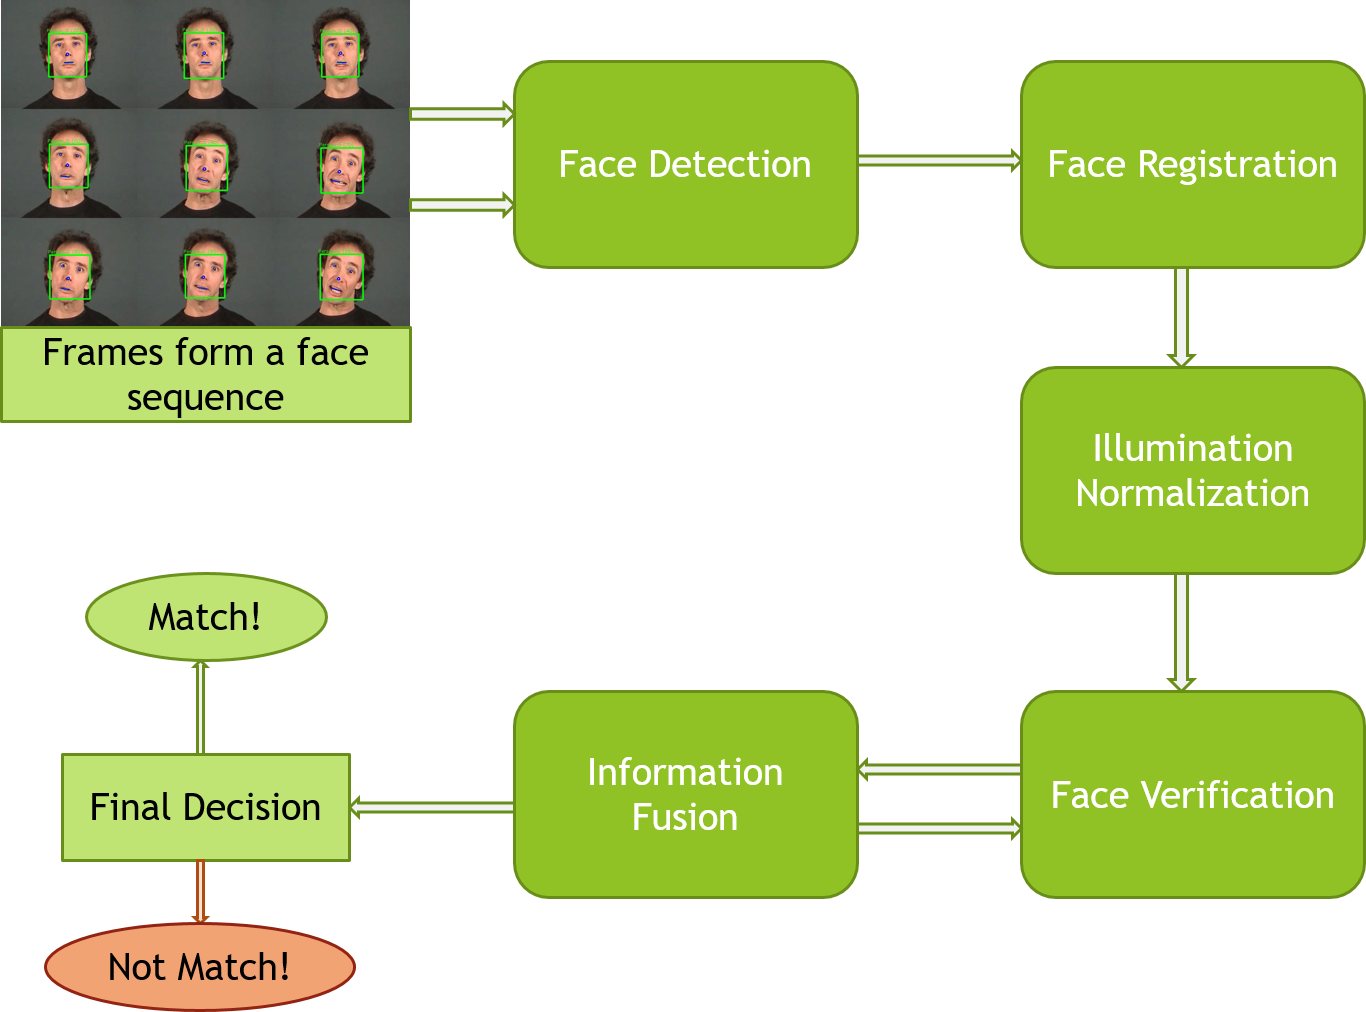
\includegraphics[width=0.9\textwidth]{img1.png}
    \end{figure}
    \end{frame}
    
    \section{Principle Component Analysis and Linear Descriminant Analysis}
    \begin{frame}
      \frametitle{Outline for Section \thesection}
      \tableofcontents[currentsection]
    \end{frame}
    
     \begin{frame}
    \frametitle{Principle Component Analysis(PCA) and \par Linear Descriminant Analysis(LDA)}
    \begin{itemize}
    \item PCA also known as \textbf{Karhunen Lower Transformation} is used to reduce the dimensionality. Its main aim is to reduce the data onto lower dimensional space also called as Eigen space by computing the Eigen values and Eigenvectors of dataset. The output of PCA is the input to LDA algorithm. It is based on Eigen value and Eigenvector.
    \item The LDA computes the scatter matrix within class and scatter matrix between class thus separating the images within class increasing the recognition rate. After calculating the weight matrix Euclidian distance is calculated.
    \item The PCA and LDA algorithms are based on an efficient computation of Eigen values and Eigenvectors. Many methods are used to compute Eigen value and Eigenvectors such as QR method, Gauss-Seidel method, Power method, Jacobi method etc. The Jacobi method is an iterative method to find eigen value and eigenvector of symmetric matrix.
    \end{itemize}
    \end{frame}     
   

    \begin{frame}
    \begin{figure}[H]
        \graphicspath{{figs/}}
        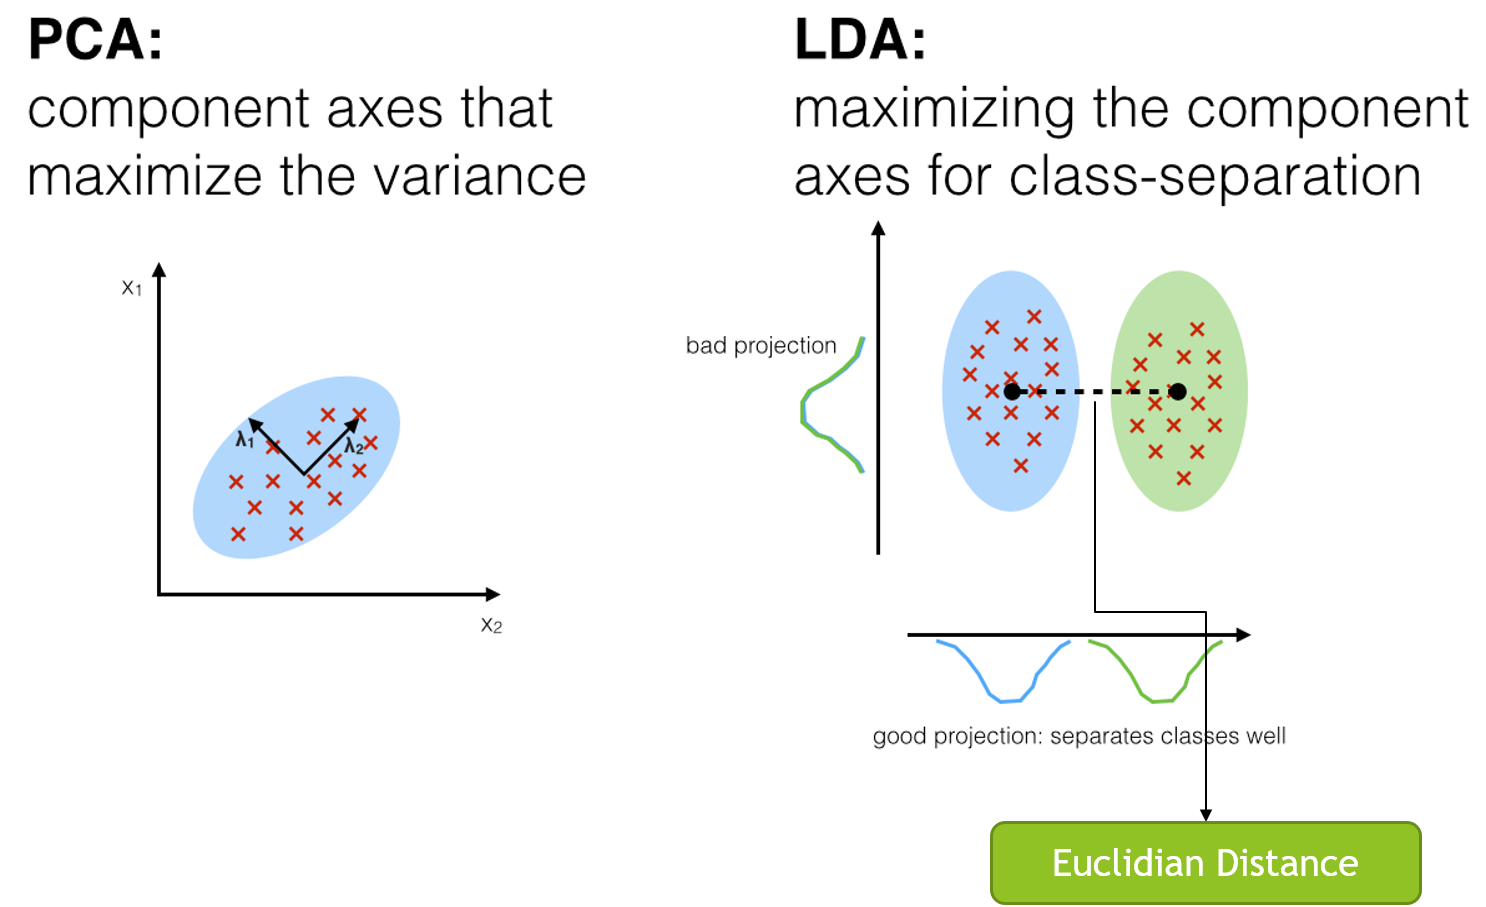
\includegraphics[width=0.9\textwidth]{img2.png}
    \end{figure}
    \end{frame}
    
     \begin{frame}
    \frametitle{Representing EigenFaces}
    \begin{figure}[H]
        \graphicspath{{figs/}}
        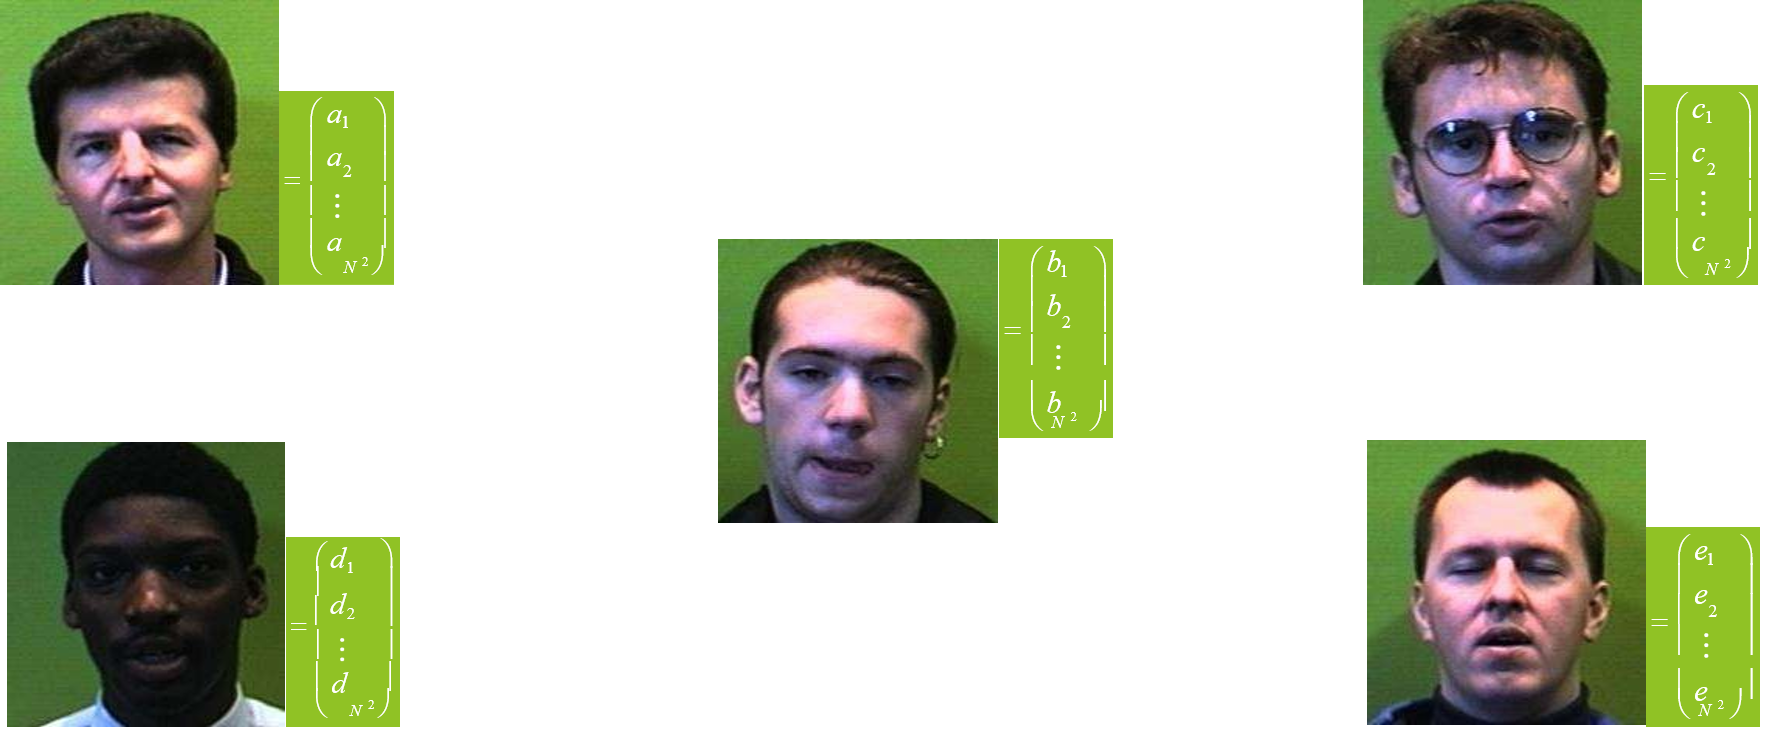
\includegraphics[width=0.9\textwidth]{img3.png}
    \end{figure}
    \end{frame}
    
    \begin{frame}
    \begin{figure}[H]
        \graphicspath{{figs/}}
        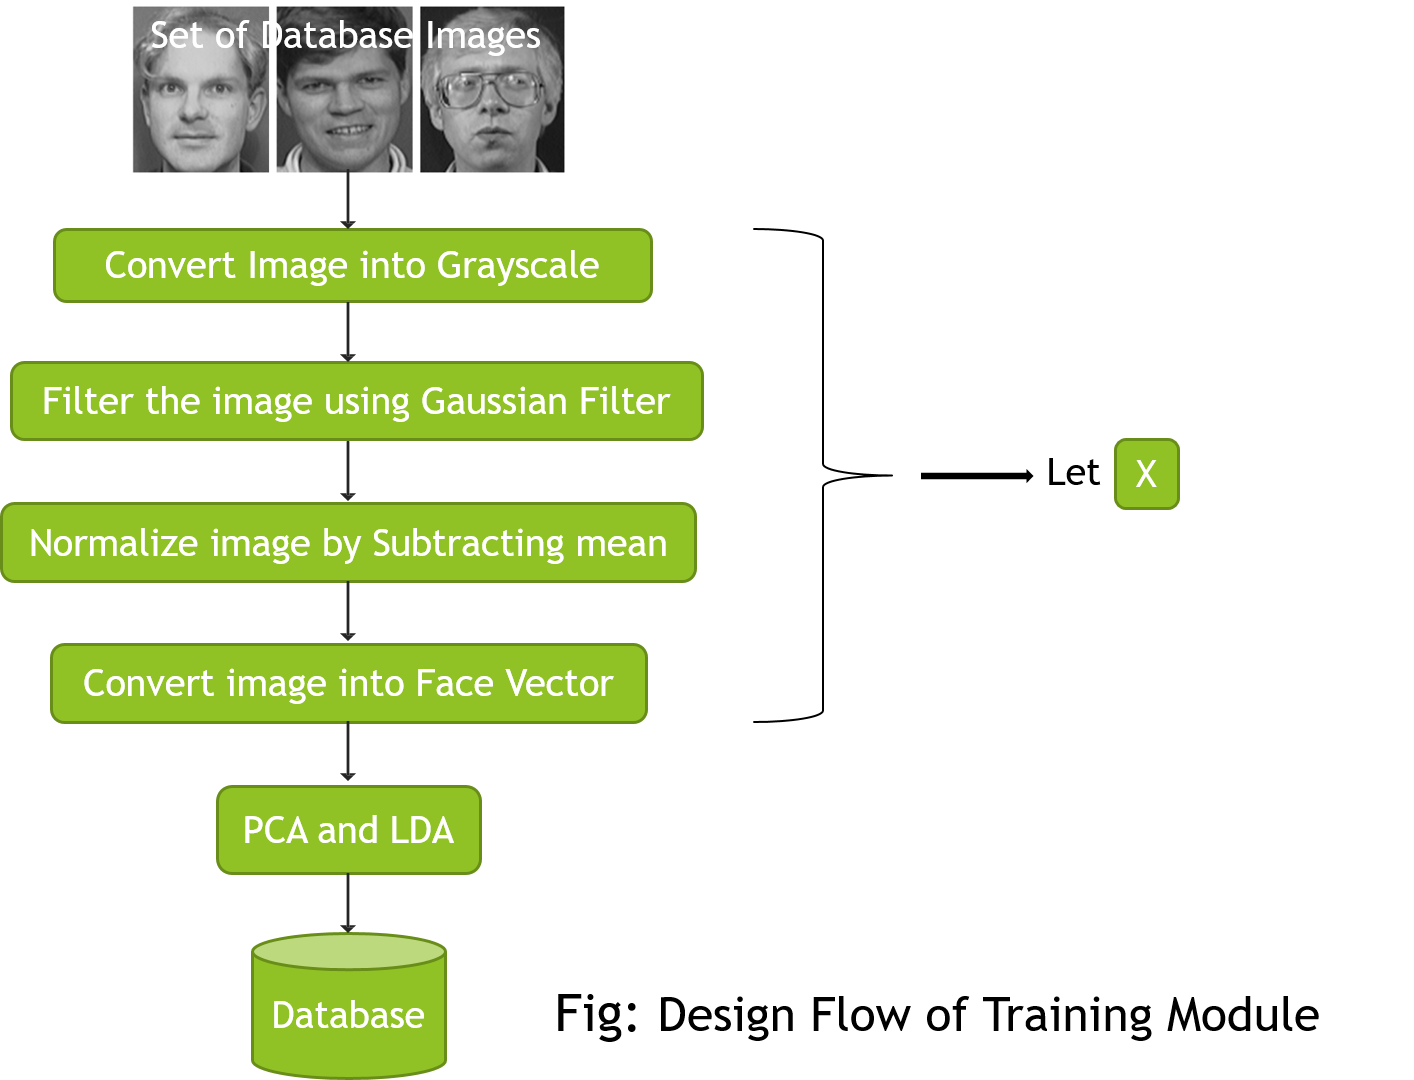
\includegraphics[width=0.9\textwidth]{img4.png}
    \end{figure}
    \end{frame}
    
      \begin{frame}
    In above Block Diagram the Training module consists of Gray scale conversion module where in all colour images are converted into Gray scale images, a Gaussian filter module to filter the image using gaussian mask, Normalisation Module by subtracting the mean of all images from each image to normalize faces, and vector conversion module that convertes 2D image are converted into 1D row vector. \newline
	Next the PCA followed by LDA algorithms are applied onto images after which database of images is obtained. This completes the Training phase of face recognition system.
       \end{frame}

    
    \begin{frame}
    \begin{figure}[H]
        \graphicspath{{figs/}}
        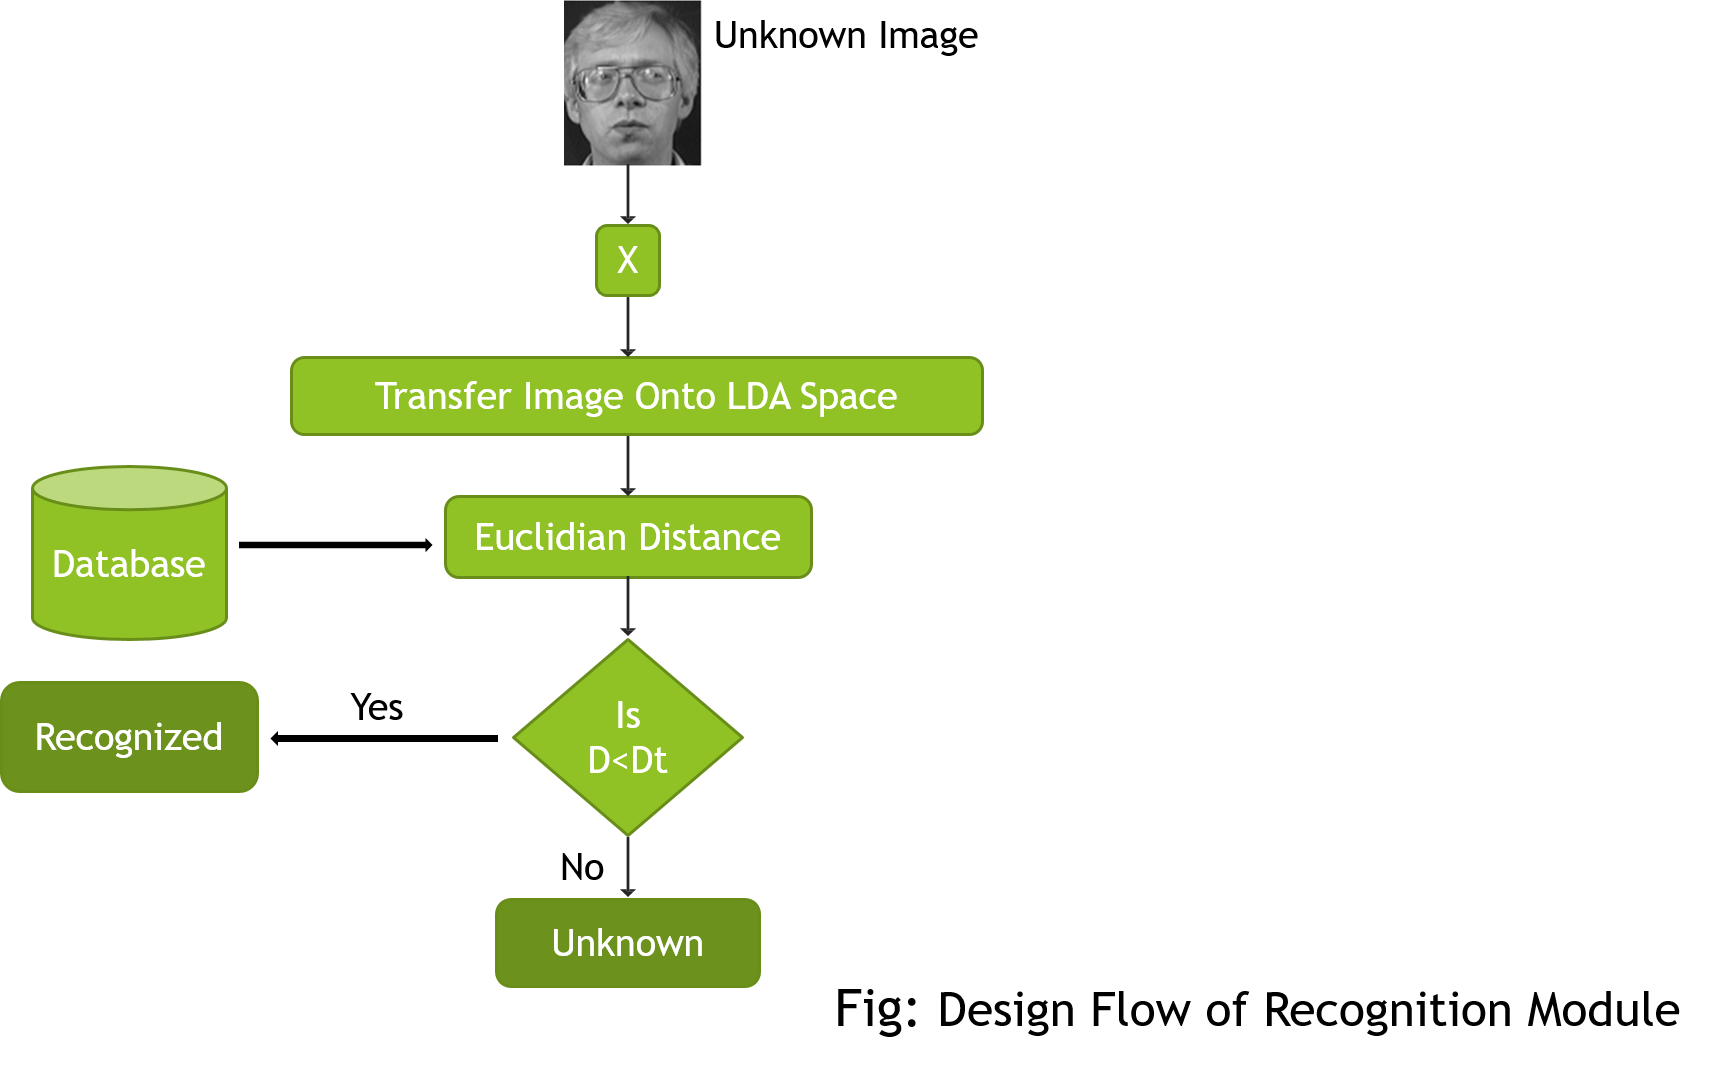
\includegraphics[width=0.9\textwidth]{img5.png}
    \end{figure}
    \end{frame}
    
     \begin{frame}
    During the recognition phase of Face Recognition system the \textbf{unknown face} is first converted into \textbf{gray scale}. Next the test image is smoothened using \textbf{Gaussian filter}. Test image is \textbf{normalized} by subtracting the mean of images from test image. Now the image is converted from 2D to 1D row and then is transferred to LDA surface space by multiplying weight of PCA and LDA. \newline

\textbf{Euclidian distance} is calculated between the LDA sub space of test image and all the LDA subspace images in the database. The minimum distance image is classified as recognized image.
       \end{frame}
       
    \begin{frame}
    \begin{figure}[H]
        \graphicspath{{figs/}}
        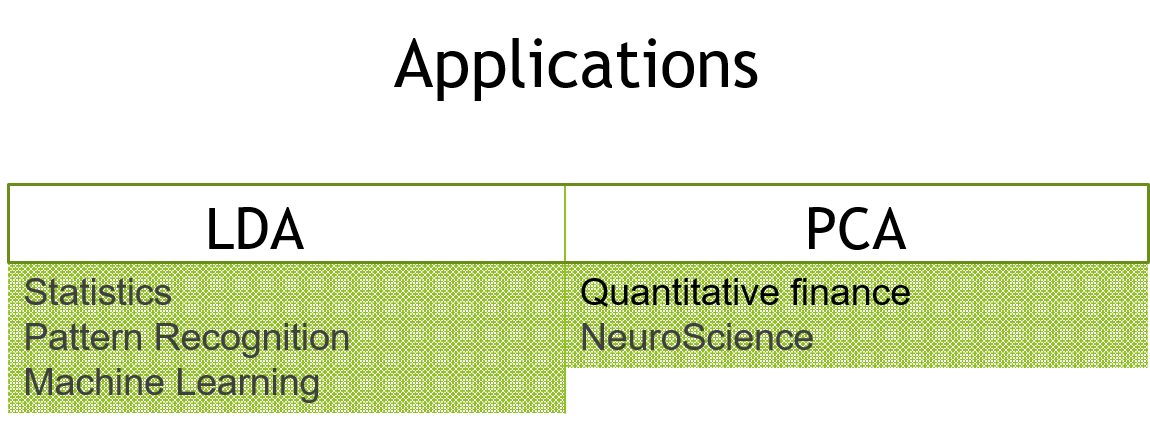
\includegraphics[width=0.9\textwidth]{img6.png}
    \end{figure}
    \end{frame}
    
    \section{Tools}
    \begin{frame}
      \frametitle{Content for Section \thesection}
      \tableofcontents[currentsection]
    \end{frame}
    
    \begin{frame}
        \frametitle{Tools}
    \textbf{Matlab}: In face detection using MATLAB program can be used to detect a face, eyes and upper body. Matlab is one of the leading software packages for numerical computation and it mainly deals with Matrices right from scalar to multidimensional matrices. Object detection and tracking are important in many computer vision applications, including activity recognition, automotive safety and surveillance. Presented here is an face detection using MATLAB system that can detect not only a human face but also eyes and upper body. \newline

\textbf{OpenCV}: OpenCV is the most popular library for computer vision. Originally written in C/C++, it now provides bindings for Python.
    \end{frame}
    
    \section{Other face recognition algorithms}
    \begin{frame}
      \frametitle{Content for Section \thesection}
      \tableofcontents[currentsection]
    \end{frame}
    
    \begin{frame}
    \frametitle{Other face recognition algorithms}
    \begin{itemize}
    \item Eigenfaces Algorithm
    \item Bayesian Classifier
    \item Gabor Wavelet Algorithm
    \item Elastic graphs  
    \end{itemize}
    \end{frame}
    
    \section{Future of face recognition}
    \begin{frame}
      \frametitle{Content for Section \thesection}
      \tableofcontents[currentsection]
    \end{frame}
    
     \begin{frame}
    \frametitle{Future Of Face Recognition}
    \begin{itemize}
    \item Some consider the problem impossible
    \item No standard way of approaching the problem
    \item Advancements in hardware and software
    \item Slow integration into society in limited environments
    \item Very large potential market  
    \end{itemize}
    \end{frame}
    
    \section{Result}	
    \begin{frame}
      \frametitle{Content for Section \thesection}
      \tableofcontents[currentsection]
    \end{frame}
    
    \begin{frame}
    \frametitle{Result}
    The accuracy of FACE RECOGNITION using PCA alone was found to be 91\%, the accuracy of LDA alone was found to be 94\% and that of proposed method was found to be 97\% when implemented on raspberry pi 3 board. 
    \begin{figure}[H]
        \graphicspath{{figs/}}
        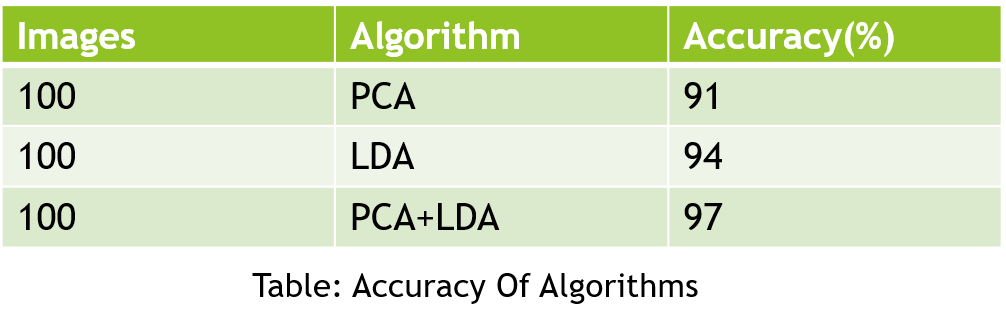
\includegraphics[width=0.9\textwidth]{img7.png}
    \end{figure}
    \end{frame}
    
    \section*{thx}
        \begin{frame}
        \begin{center}
        \fontsize{30pt}{\baselineskip}\selectfont \structure{Thank You!}
        \end{center}
        \begin{reference}{0mm}{80mm}
        \end{reference}
        \end{frame}
\end{document}
